\documentclass[conference]{IEEEtran}
\usepackage{amsmath}
\usepackage[pdftex]{graphicx}
\usepackage{gensymb}
\usepackage{biblatex}
\addbibresource{bibliography.bib}
\usepackage{hyperref}
\usepackage{url}
\hyphenation{op-tical net-works semi-conduc-tor}

\begin{document}
\title{\Large \bf G2G - Disentanglement by Cross-Training}
\author{
\IEEEauthorblockN{Li Nguyen, ID: 934644485}
\IEEEauthorblockA{Department of Informatics\\Technical University of Munich\\
li.nguyen@tum.de}

\and
\IEEEauthorblockN{Alexander Koenig, ID: 918254061}
\IEEEauthorblockA{Department of Informatics\\Technical University of Munich\\
awc.koenig@tum.de}
}
\maketitle
\begin{abstract}
Disentanglement is often considered as one of the most challenging tasks in modern machine learning. In this project, we propose the G2G architecture, which aims to solve the disentanglement task by cross-training: in a disassembly stage, the content and class information of two original images is separated. Subsequently, two images are generated by mixing the previously isolated information. This mixing process is then repeated in a reassembly stage. Ideally, the overall process should yield reconstructions that are similar to the original images. We compare three independent approaches to implement the G2G architecture. A naive approach with symmetric encoders and a simple decoder lacked generative power. A second approach which is based on the FUNIT architecture with a CycleGAN discriminator failed to produce disentangled images. In a third approach, we used pre-trained FUNIT networks and demonstrated that the G2G concept produces sensible outputs in a forward pass. However, resuming training to produce higher quality images proved to be challenging. 

Code is available at \url{https://github.com/axkoenig/ml4cg} (for the first two approaches) and   
\url{https://github.com/nichtwegzudenken/ml4cg} (for the third approach)\end{abstract}.

Keywords: Machine Learning, Computer Graphics, Disentanglement, Generative Adversarial Networks
\IEEEpeerreviewmaketitle

\label{chap1_introduction}
\section{Introduction}
Disentanglement with deep neural networks remains one of the main research challenges of modern machine learning. A disentangled representation separates an original representation into disjoint parts and allows for the independent control of one or more of these separated features. Disentanglement plays a large role at the intersection of machine learning and computer graphics as it is often beneficial to separate images into meaningful and independent features for further processing. For example, an image of a car may be separated into different feature representations such as "color", "type", "pose", "rest". 

A branch of deep learning where the separation of information is especially beneficial is that of generative adversarial networks (GANs). These networks were originally proposed by Goodfellow et al. \cite{goodfellow2014generative}. The main idea behind GANs relies on adversarial training of a generator and discriminator: The discriminator aims at distinguishing whether an image is fake or real while the generator tries to maximize the probability of the discriminator classifying the fake image as real and thereby creates more realistic outputs. It was shown that GANs can use disentangled representations to recreate new images. By altering one or more of the disentangled representations this will directly relate to the generated image (e.g. by manipulating the "pose" feature from the car example, the car can be visualized in different poses). 

Disentanglement systems in combination with generative networks can be used for image editing and generating artificial datasets. For example, this can be beneficial in the medical domain where only a limited amount of X-ray images of a tumor in a specific location exist. A disentanglement approach could be trained to separate the "location" attribute and a generative adversarial network could sample within this attribute and recombine it with the "rest" attribute of the original image to create a new image. Thus, an existing dataset could be enhanced which may improve consequent algorithms. 

\label{chap2_related_work}
\section{Related Work}

Disentangling features without any supervision remains an ongoing research challenge. Furthermore, fully supervised disentanglement is often a cumbersome task due to the lack of labeled data. For example for the task of transferring the gender of a facial image, there is rarely an image of the same person in another gender. This also applies to image-to-image translation as seen in CycleGAN \cite{zhu2017unpaired}. Consequently, most state-of-the-art approaches incorporate supervision but as little as possible. Many related works include class-supervision, which means that only the class labels for each image in the training set are given. The majority of related projects try to disentangle in a two-fold fashion by disentangling one class feature (e.g. the identity of a person) from the content features which often represent the rest of the photo, such as pose, facial expression, lighting, and the background \cite{nitzan2020disentangling} \cite{liu2019few} \cite{mokady2019mask}. 
From an architectural standpoint, most of the existing approaches leverage adversarial training.

% FUNIT
For example, Liu et al.'s FUNIT (Few-Shot Unsupervised Image-to-Image Translation) maps "images in a given class to an analogous image in a different class" \cite{liu2019few}. They use a discriminator which discriminates between original input images and synthetically generated images. This should encourage the generator to enhance image quality and realism. 
They use a subset of the ImageNet ILSVRC2012 training set by only extracting faces of different animals and use one or more class images for translating into an analogous image of an unseen target class, hence the name \textit{Few Shot Image to Image Translation}. The approach has one class and one content encoder which produce latent class and content codes of the respective images. The class code is then fed into the generator through AdaIN layers, which were originally proposed by Huang and Belongie \cite{huang2017arbitrary}. The content code is directly fed into the generator and the combination of both codes gives the translated image. This works well with images of good quality and facial poses which are not too complex, however, with facial close-ups, the approach still struggles to generate realistic outputs.

% Fader Networks
Lample et al. use adversarial training a little bit differently: They also use an encoder-decoder architecture but let the discriminator act on the latent space rather than directly on the images.
Their goal is to produce an attribute-invariant latent representation, which should encode the "rest" of an image, such as background, lighting, and pose to be able to feed the generator a new and altered attribute to generate an image using the altered attribute.
To do this their discriminator tries to "guess" the attribute which is encoded inside the latent code of an image. As their goal is to obtain an attribute-invariant latent representation, the discriminator should prohibit the generator from encoding any attributes. The latent code thus only contains the "rest of the image". This should prohibit the decoder from reconstructing the image using the original attribute $y$, resulting in the same original image, but use an altered attribute $y'$ to create a new image \cite{lample2017fader}.
Their approach also allows for altering the \textit{intensity} of the attribute because the attribute values for the altered attributes are continuous. This also gives the project the name \textit{fader networks} as the faders on a mixing console can also be used to adjust the intensity of channels.

% Ron's Paper
Another approach using adversarial training is the one by Mokady et al. which translates attributes in a weakly supervised manner. Their approach makes it possible to seamlessly transfer content that exists in sample $b$ of the domain $B$ onto a sample $a$ of another domain $A$, e.g. a pair of glasses or a mustache is transferred from one face to another. They do this by generating a mask that outlines the shape of the attribute, e.g. the glasses or the mustache.
Their architecture incorporates two encoders -- one for the \textit{separate} attribute (glasses, moustache) and one for the \textit{common} ones, i.e. the rest of the image. 
The common encoder aims at capturing the common (and domain invariant) information between the domains A and B, while the separate encoder encodes only the separate attribute.
A discriminator tries to distinguish between the common code of domain A and B, while the common encoder tries to produce latent codes which are indistinguishable for the discriminator. Ideally, the common code is the same for both domains such that the separate attribute is not encoded. Their results show very realistic translations and even allow for altering the separate attribute such as changing the style of the glasses.

% Yotam's Paper
Very promising results for disentanglement in human faces come from Nitzan et al. which successfully manage to disentangle the identity of a person from the rest of the image features. They obtain high visual quality by harnessing the pre-trained unconditional image generation network StyleGAN by Karras et al. \cite{karras2019style}.
Nitzan et al. have minimal supervision and decouple the process of disentanglement and synthesis. They tackle the disentanglement in their project and outsource the process of synthesis to the pre-trained StyleGAN. First, they map the images into a latent space $Z$ using two encoders $E_{id}$ and $E_{attr}$ -- the former encodes the identity $f$ and the latter the rest $f'$. Using a network $M$, they map this code into the latent space $W$ of the pre-trained generator $G$ and thereby leverage the state of the art power of StyleGAN. They map into Z first and not directly into W because the Z-space is more disentangled. As the mapping from $Z$ into $W$ is not trivial, they introduce a discriminator $D_W$ which tries to distinguish the real encodings from StyleGAN’s $W$-space and their own network $M$’s mappings. Using this method they are even able to alter the hair belonging to the identity of the person, which other approaches were not capable of.

% LORD
One of the few projects which does not use adversarial training is LORD by Gabbay and Hoshen. LORD stands for Latent Optimization for Representation Disentanglement and presents a universal formulation for class and content disentanglement. They train in a class-supervised setting and propose two main contributions for disentanglement. 
They perform \textit{Shared Latent Optimization}: The class representations are modeled as embeddings which should ideally be identical for images of the same class. This should prevent content information from being encoded inside the class representation. Furthermore, they use \textit{Asymmetric Noise Regularization} by which they "want to make sure that no class information leaks into the content representation" \cite{gabbay2019demystifying}. They regularize the content code to enforce the minimality of information.

\label{chap3_data}
\section{Datasets}

\subsection{Naive Approach and CycleFUNIT Approach}
The disentanglement of human faces remains an ongoing challenge. This is partly due to the fact that we humans are very sensitive to even the slightest irregularities in faces, which makes it hard to generate realistic-looking images of faces. Therefore, we want to address this challenge and work on the CelebA dataset \cite{liu2015faceattributes} in our first and second approach (i.e. the naive and the CycleFUNIT approach).

\subsection{FUNIT2FUNIT Approach}
For our third approach -- which we call FUNIT2FUNIT -- we extended the FUNIT model by embedding it into our own architecture. For this purpose, we use the pre-trained network provided by Liu et al. \cite{liu2019few}, which was trained on animal faces. Hence, we use the animal face dataset which was also used by Liu et al. and is a subset of the ImageNet ILSVRC2012 training set \cite{imagenet_cvpr09}.

\section{Methods}

The idea of this research project is the so-called G2G architecture. In this architecture there are two generative stages: In the first stage, two attributes of each input image are isolated and then recombined into a new image with mixed attributes. By repeating this mixing process in the second stage, both output images should ideally be a perfect reconstruction of the original input images (see figure \ref{fig:g2g_arch}). The research question is whether this architecture can evoke and facilitate disentanglement.

\begin{figure*}[h!]
	\centering
	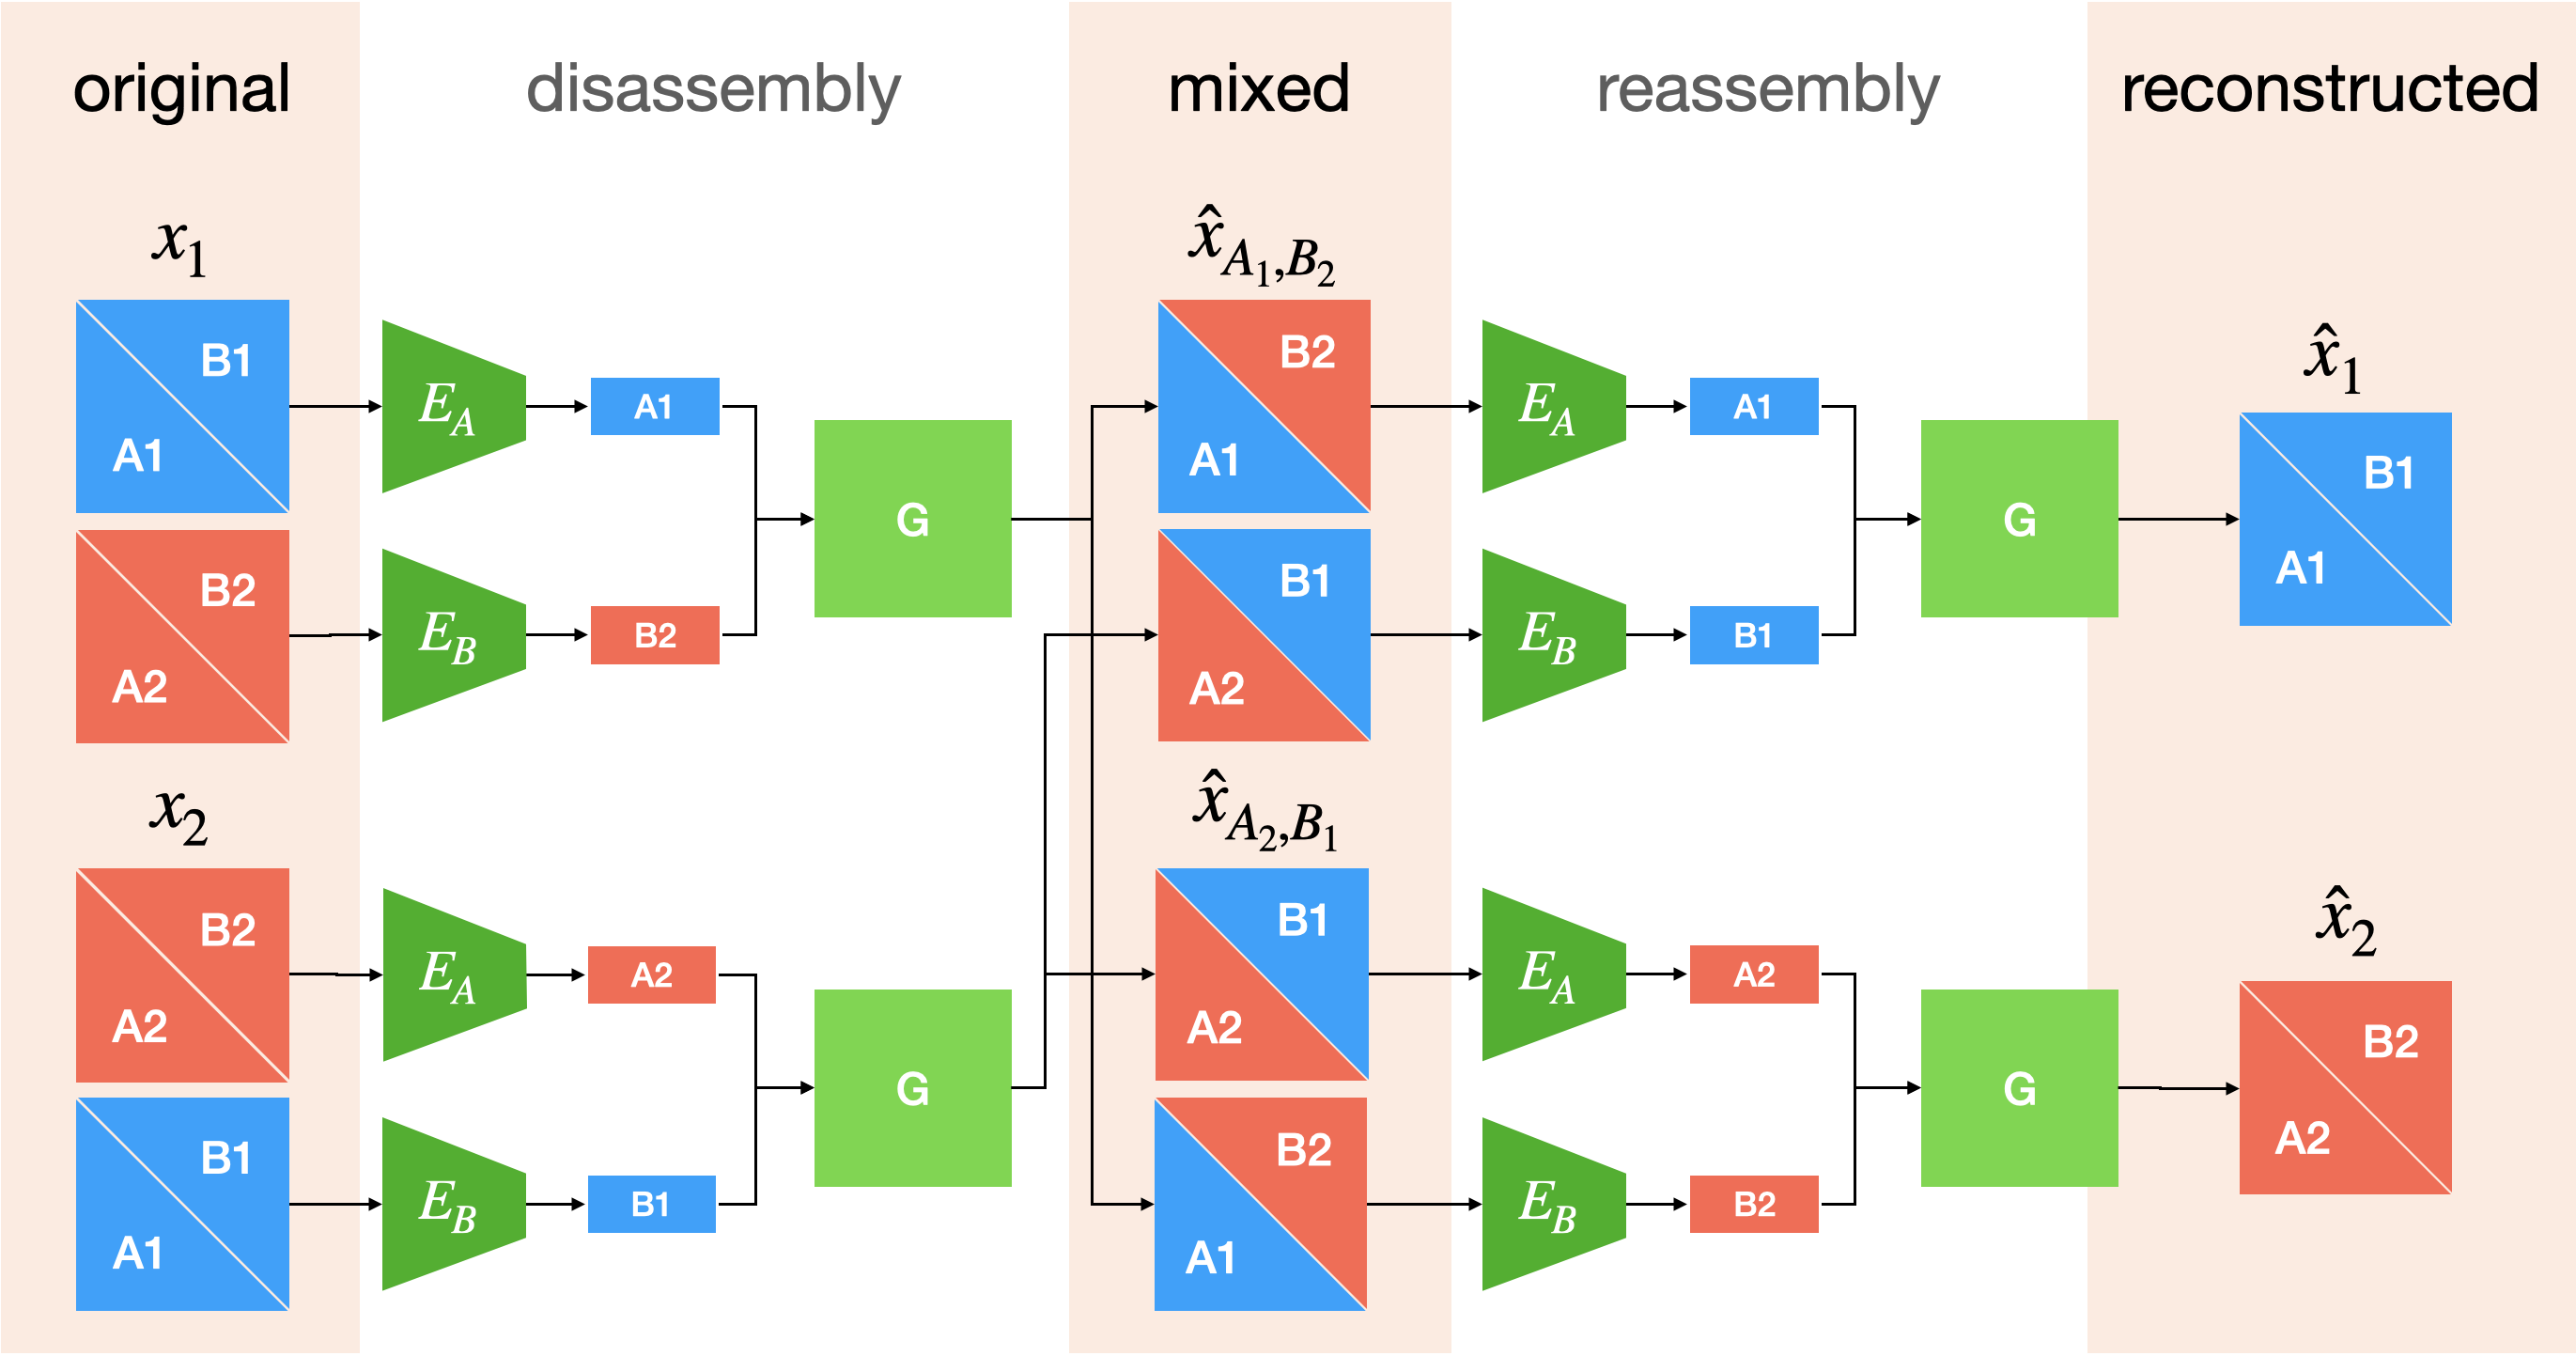
\includegraphics[width=0.9\textwidth]{figures/g2g_arch.png}
	\caption{Scheme of the two-staged G2G architecture}
	\label{fig:g2g_arch}
\end{figure*}

Let $x_1$ and $x_2$ denote the blue and red input images seen in figure \ref{fig:g2g_arch}. In this project we try to disentangle one separate attribute -- the \textit{class} feature -- from the \textit{rest} of the image -- the content feature. The class information corresponds to the identity of a person in the CelebA dataset. Encoder $E_A$ should encode the rest of the image, such as pose, facial expression, background, lighting, etc. while encoder $E_B$ encodes the class. Ideally, no information of the class code $B1$ should leak into code $A1$ and vice versa. The generator $G$ should learn to stitch the two codes together and generates a new and mixed image which should have the identity $B2$ and the \textit{rest} information of $A1$ (compare figure \ref{fig:g2g_arch}). The mixed images $\hat{x}_{A1,B2}$ and $\hat{x}_{A2,B1}$ which we obtain from this first stage are then fed into the same encoders again: The \textit{class} and \textit{rest} latent codes are extracted and new images are generated from it, which should result in perfect reconstructions $\hat{x}_1$ and $\hat{x}_2$.

In the following, we present three independent approaches by which we implement the G2G architecture. The research question at hand is whether disentanglement can be enhanced with the G2G architecture while keeping supervision as minimal as possible.
We start off with a naive approach, with a straight-forward architecture for the generator and both encoders. 
Further, we implement a second approach in which the encoder and decoder parts are taken from the FUNIT project of Liu et al. and the discriminator was taken from Zhu et al.'s CycleGAN \cite{zhu2017unpaired}.
In a third approach, we assemble a pre-trained FUNIT model in the G2G architecture and resume training to check if the G2G architecture can outperform the vanilla FUNIT approach.

\subsection{Naive Approach}

For the naive approach, we constructed two symmetric encoders $E_A$ and $E_B$ which are inspired by Mokady et al. \cite{mokady2019mask}. The generator was taken from Gabbay and Hoshen \cite{gabbay2019demystifying}. One of the latent codes is fed into the generator directly, while the other is fed in via AdaIN layers. For supervision we introduce the reconstruction loss in equation \ref{eq:naive_recon} and two cycle consistency losses, one for each code (see equations \ref{eq:naive_cycle_b} and \ref{eq:naive_cycle_a}). The reconstruction loss is motivated by the fact that the original images should be as similar as possible to the reconstructed images. The cycle consistency losses should guide the network to produce the same low-dimensional embeddings in the disassembly stage as in the reassembly stage (e.g. the feature code $A_1$ should be the same from original image $x_1$ as from the mixed image $\hat{x}_{A_1, B_2}$). The overall loss function for the generative network is stated in equation \ref{eq:naive_all}.

\begin{equation}
	\mathcal{L}_{r} = \sum_{i=1}^{n} \left\| \hat{x}_i - x_i \right\| 
	\label{eq:naive_recon}
\end{equation}

\begin{equation}
\begin{split}
\mathcal{L}_{cyc, E_A} = \sum_{i=1}^{n-1} 
\left\| E_A(x_i) - E_A(\hat{x}_{A_i,B_{i+1}}) \right\|^2 + \\
\left\| E_A(x_{i+1}) - E_A(\hat{x}_{A_{i+1},B_i})
\right\|^2
\label{eq:naive_cycle_a}
\end{split}
\end{equation}

\begin{equation}
\begin{split}
\mathcal{L}_{cyc, E_B} = \sum_{i=1}^{n-1} 
\left\| E_B(x_i) - E_B(\hat{x}_{A_{i+1},B_i}) \right\|^2 + \\
\left\| E_B(x_{i+1}) - E_B(\hat{x}_{A_1,B_{i+1}}) \right\|^2
\end{split}
\label{eq:naive_cycle_b}
\end{equation}

\begin{equation}
	\mathcal{L}_{all} = \mathcal{L}_r + \gamma \cdot \big( \mathcal{L}_{cyc, E_A} + \mathcal{L}_{cyc, E_B} \big)
	\label{eq:naive_all}
\end{equation}

\subsection{CycleFUNIT}
The second approach, which we refer to as \textit{CycleFUNIT}, is a combination of the encoders and decoders of Liu et al.'s FUNIT \cite{liu2019few} and the CycleGAN objective by Zhu et al. \cite{zhu2017unpaired}. The FUNIT content encoder should encode the global style of the image such as pose, background, and facial expression, while the FUNIT class encoder should encode the person's identity. The FUNIT decoder replaces our generator $G$. 

Since we had problems with image quality in the naive approach, we conducted a simple sanity check before proceeding with architectural considerations. To validate that the FUNIT architecture is capable of generating high-quality images, we fed the network depicted in figure \ref{fig:funit_block} with two identical images and guide it to reconstruct the input image. As a reconstruction loss we used the VGG perceptual loss of a VGG16 \cite{johnson2016perceptual} (see equation \ref{eq:cyclefunit_recon}). Our experiments were successful: the FUNIT architecture gave us a perfect reconstruction with high image quality.

\begin{figure}[h!]
	\centering
	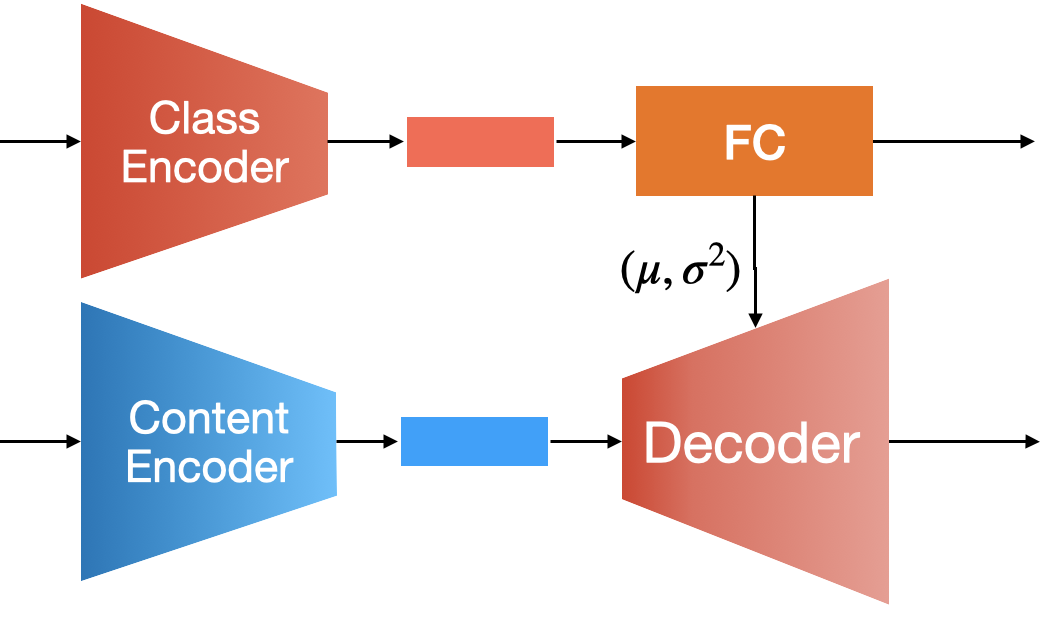
\includegraphics[width=0.7\linewidth]{figures/FUNIT_block.png}
	\caption{Architecture of the FUNIT network by Liu et al. \cite{liu2019few}}
	\label{fig:funit_block}
\end{figure}

\begin{equation}
	\mathcal{L}_{VGG} = \sum_{i=1}^{n} \left\| E_{VGG} \big( \hat{x}_i \big) - E_{VGG} \big( {x}_i \big) \right\| ^2
	\label{eq:cyclefunit_recon}
\end{equation}

After achieving high visual quality in the sanity check, we integrate the FUNIT architecture into the G2G structure we presented above. We add the cycle consistency losses in equations \ref{eq:naive_cycle_a} and \ref{eq:naive_cycle_b} which we also used in the naive approach. Further, we add the "long" VGG reconstruction loss in equation \ref{eq:cyclefunit_recon}. Note that "long" always refers to "from original to reconstructed image" while a loss loss "from original to a mixed image" would be referred to as "short".

To enhance the image quality of the mixed images we add the discriminator from CycleGAN which introduces a third type of loss. The discriminator takes the original images and the mixed images and tries to distinguish between real (original) and fake (mixed) ones while the generator tries to fool the discriminator by producing more realistic outputs.
Let $S_g$ be the set of generated (mixed) images and $S_o$ the set of original images. Then the generator tries to generate images that are classified as 1, i.e. real (see equation \ref{eq:cyclefunit_gen}). On the other hand, the discriminator tries to differentiate between real and fake images (compare equation \ref{eq:cyclefunit_disc}). 
The overall loss of stage two therefore contains the reconstruction and cycle consistency losses \ref{eq:cyclefunit_recon}, \ref{eq:naive_cycle_a} and \ref{eq:naive_cycle_b} and the losses \ref{eq:cyclefunit_gen} and \ref{eq:cyclefunit_disc} for the generator and discriminator.

\begin{equation}
	\mathcal{L}_{G} = \frac{1}{|S_m|} \sum_{x \in S_m} l \big( D (x),1 \big) 
	\label{eq:cyclefunit_gen}
\end{equation}

\begin{equation}
	\mathcal{L}_{D} = \frac{1}{|S_m|} \sum_{x \in S_m} l \big( D (x),0 \big) + \frac{1}{|S_o|} \sum_{x \in S_o} l \big( D (x), 1 \big)
	\label{eq:cyclefunit_disc}
\end{equation}

To encourage disentanglement we also add a pre-trained identity encoder. We leverage a pre-trained face detector as an identity encoder by removing its last prediction layer. The network is a ResNet-50 \cite{he2015deep} and it was pre-trained on the VGGFace2 dataset \cite{cao2017vggface2}. If two images show a person with the same identity, then this face detection network should give a similar latent identity code for both images. 
We conduct two separate experiments with the identity encoder. Firstly, we obtain the identity code of the mixed images and minimize the L1 distance between the original and its corresponding mixed image (see equation  \ref{eq:cyclefunit_id}). In this way, we want to provide the network with a further incentive to swap the identities of both persons.

\begin{equation}
\begin{split}
	\mathcal{L}_{ID} = \sum_{i=1}^{n-1} \left\| E_{ID} \big( x_i \big) - E_{ID} \big(\hat{x}_{A_i, B_{i+1}} \big) \right\| + \\ \left\| E_{ID} \big( x_{i+1} \big) - E_{ID} \big(\hat{x}_{A_{i+1}, B_i} \big) \right\|
	\label{eq:cyclefunit_id}
\end{split}
\end{equation}

Secondly, we conduct a separate experiment where we replace the encoder $E_B$ with the pre-trained identity encoder. We do not enforce the loss from equation \ref{eq:cyclefunit_id} in this case. 

\subsection{FUNIT2FUNIT 
\label{chap4_methods_FUNIT2FUNIT}}
\label{sub:funit2funit}
To assess the effect of the G2G architecture more precisely we assemble a pre-trained network into the G2G architecture. For this purpose, we use the pre-trained FUNIT architecture which was also utilized in the CycleFUNIT approach and attempt to refine the weights by continuing training. FUNIT originally is a few-shot approach -- i.e. it can take multiple class images as input. However, in our case, we use it for one-shot image generation to ensure comparability to the other approaches. The authors of the FUNIT paper showed that their network produces sensible results for the one-shot case. The overall architecture of the FUNIT2FUNIT approach is depicted in figure \ref{fig:funit2funit}.

\begin{figure*}
	\centering
	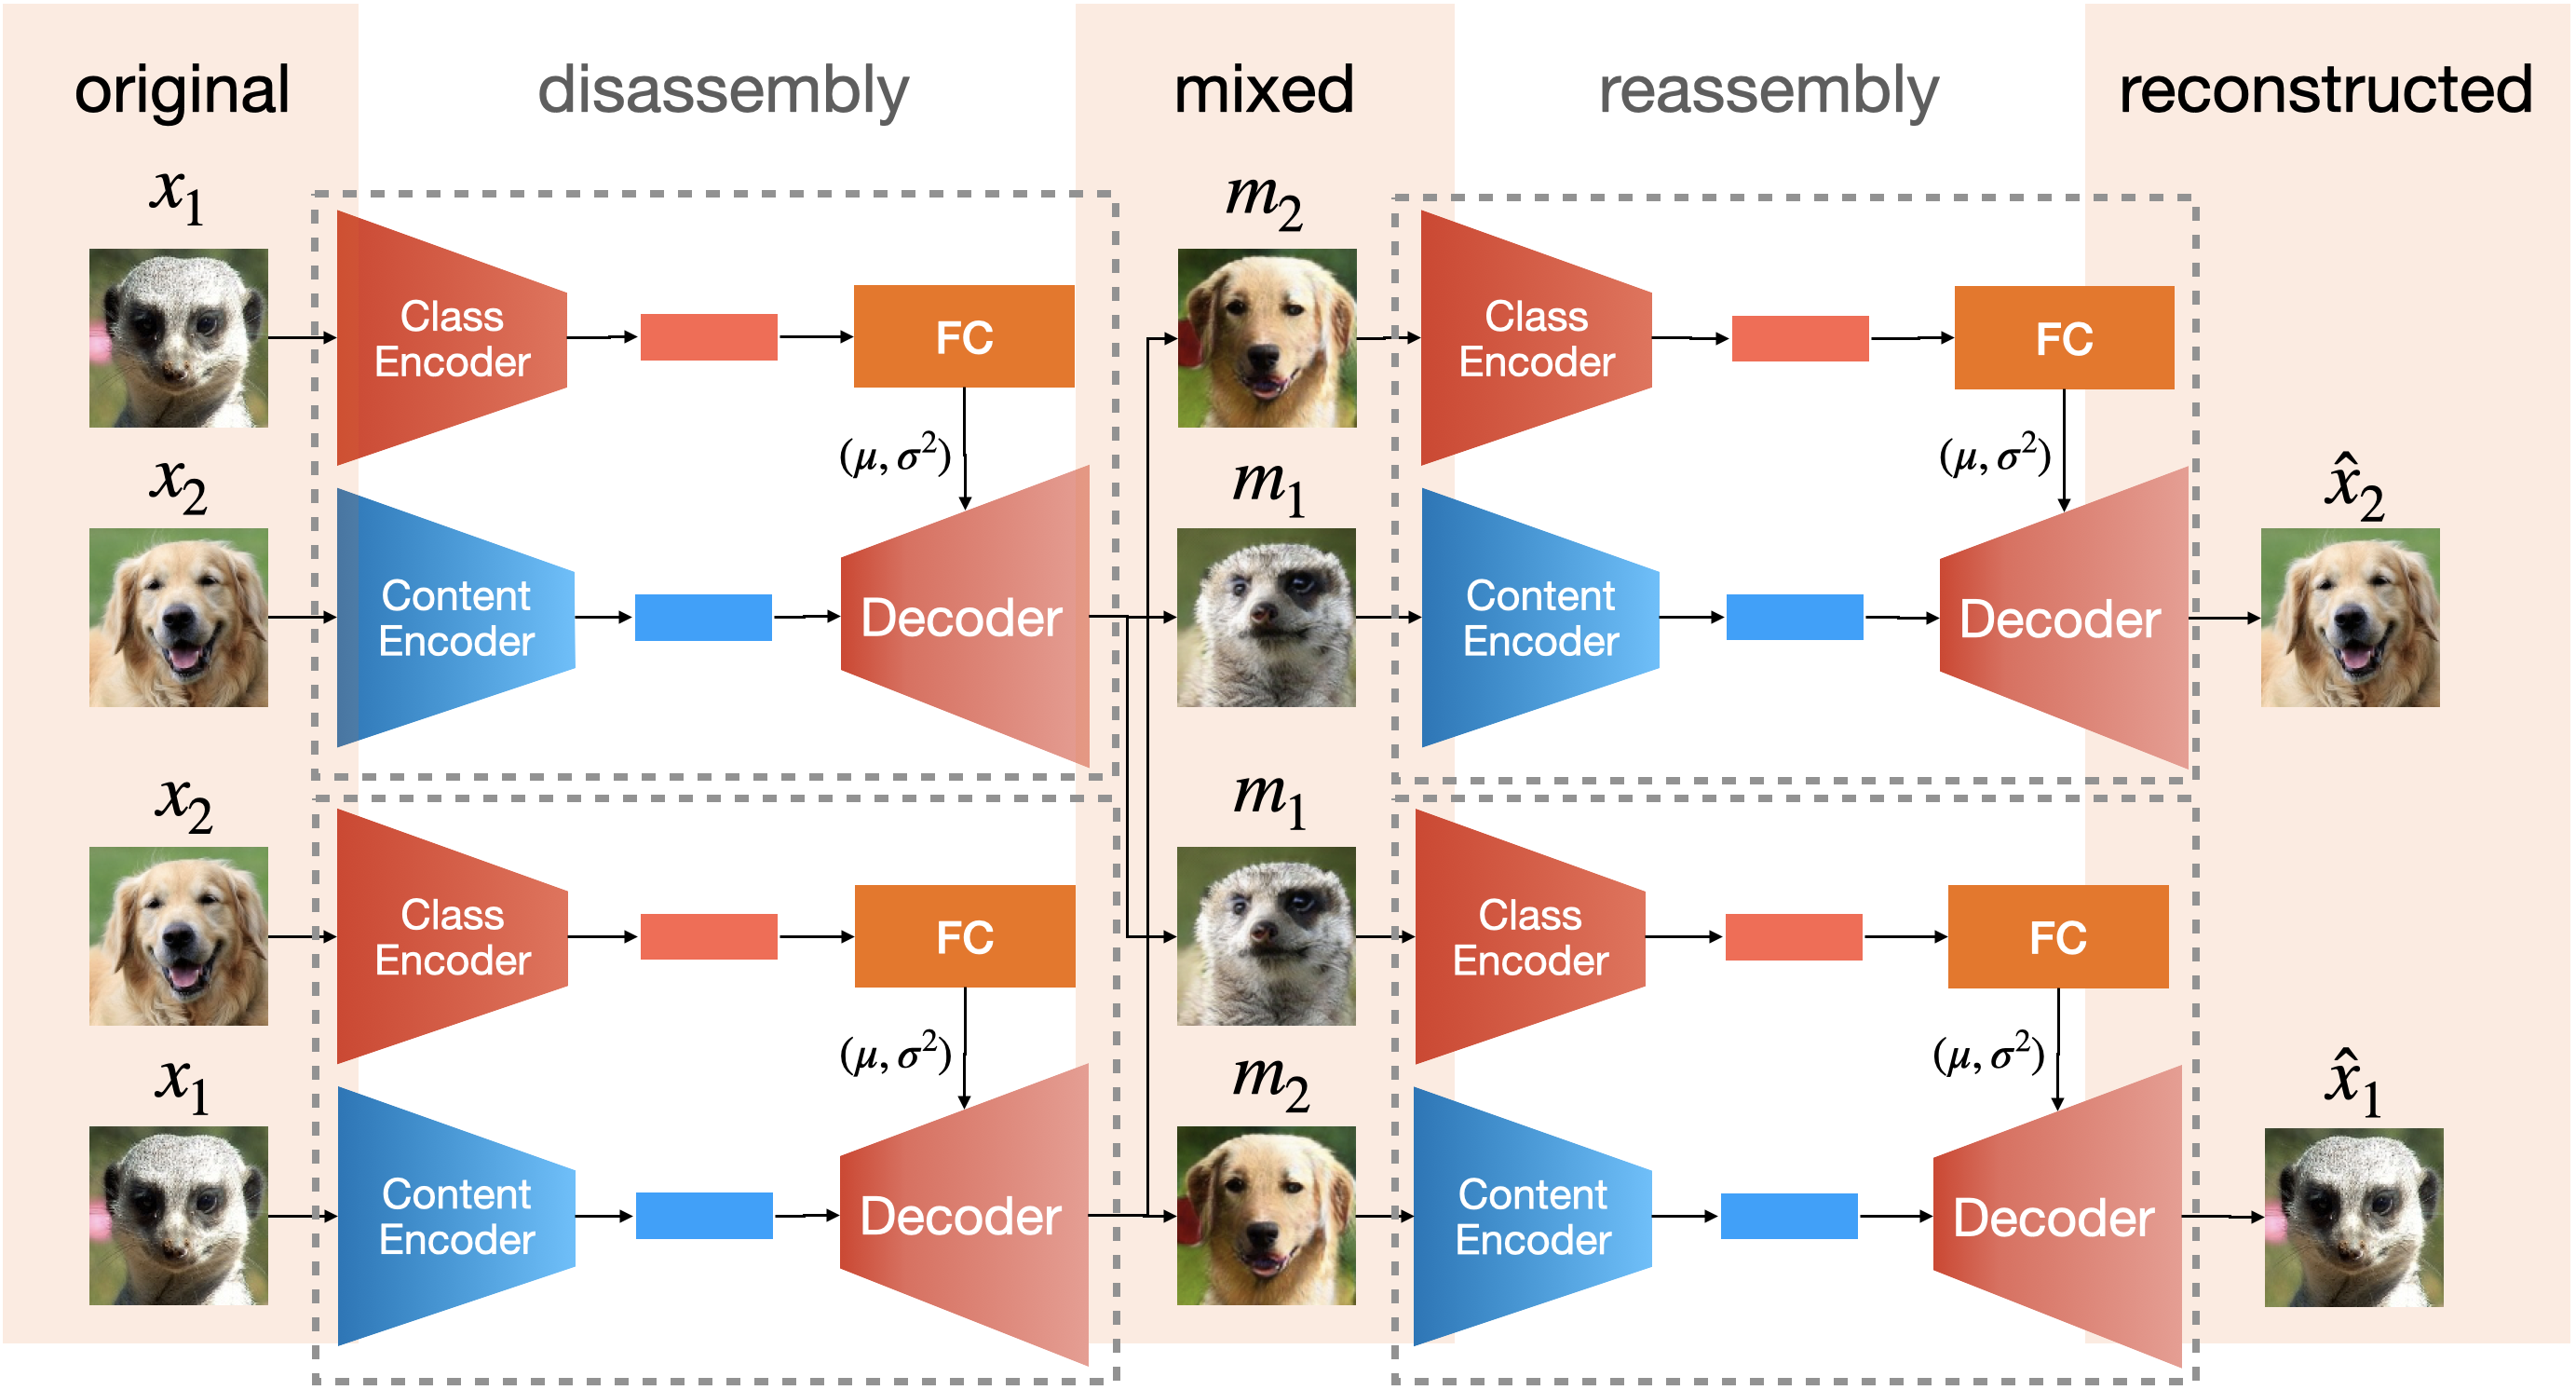
\includegraphics[width=\textwidth]{figures/funit2funit.png}
	\caption{FUNIT2FUNIT: Embedding FUNIT into the G2G architecture (with desired reconstruction images)}
	\label{fig:funit2funit}
\end{figure*}

The losses that are used in the original FUNIT approach are a GAN loss, a reconstruction loss, and a feature matching loss. Similar to our previous strategy a discriminator is fed both original and the generated images and tries to distinguish between fake and real images. The generator is thereby encouraged to produce more realistic and high-quality images. This FUNIT adversarial loss is left unchanged for the FUNIT2FUNIT approach (for details see \cite{liu2019few}).

The reconstruction loss is a "short" L1 loss between an original image that is fed into both FUNIT encoders and the reconstructed image. The reconstruction loss of the original FUNIT approach uses only the content image. In this project, we also use the class image for the short reconstruction loss to get more data through the network before an update step occurs. Note that the "short" reconstruction loss is only applied in the disassembly stage to avoid training on non-realistic looking images in the reassembly stage. 
Furthermore, we add a "long" reconstruction loss over the whole G2G architecture. In figure \ref{fig:funit2funit} this equals to minimizing the L1 distance between $x_1$ and $\hat{x}_1$ and $x_2$ and $\hat{x}_2$. We therefore get the following overall reconstruction loss with $G(a,b)$ being one FUNIT sub-network as depicted in figure \ref{fig:funit_block} with the class image $a$ and content image $b$.

\begin{equation}
\begin{split}
	\mathcal{L}_{R} = \sum_{i=1}^{n-1}  \lambda_{short} \left\| x_i - G(x_i,{x_i}) \right\| +\\ \lambda_{long}
	\left\| x_i - G(m_i,m_{i+1}) \right\| 
	\label{eq:funit2funit_rec}
\end{split}
\end{equation}

The feature matching loss uses the discriminator which is used for the GAN loss at the same time. Here, the discriminator extracts the features of an original class image and the mixed image of the same class. The L1 distance between these feature codes is minimized. To illustrate this with an example, imagine inputting the meerkat $x_1$ and the dog $x_2$ seen in figure \ref{fig:funit2funit}. Then the images of the meerkat and the ones of the translated meerkat $m_1$ in the pose of the dog are fed into the discriminator and the distance between the feature codes is minimized to enforce a high-level similarity of both images.
Again, we extend the feature matching loss for the G2G architecture. We use the vanilla FUNIT feature matching loss for the disassembly stage and reassembly stage. In the reassembly stage, we measure the distance between the features of e.g. the dog $m_2$ in figure \ref{fig:funit2funit} and the ones of the reconstructed dog $\hat{x}_2$.
Lastly, the features between the original and the fully reconstructed images can also be matched, which gives the  total feature matching loss in equation \ref{eq:funit2funit_fm}. 

\begin{equation}
\begin{split}
	\mathcal{L}_{FM} = \sum_{i=1}^{n-1} \lambda_{D} \left\| D_f(x_i) - D_f(m_i) \right\| + \\
	 \lambda_{R} \left\| D_f(m_i) - D_f(\hat{x}_i) \right\| + \\ \lambda_{L} \left\| D_f(x_i) - D_f(\hat{x}_i) \right\| 
	\label{eq:funit2funit_fm}
\end{split}
\end{equation}

Similarly, we modified the loss for the discriminator. FUNIT implements a loss for real and fake samples. In the FUNIT approach only the class image and its respective mixed image are fed through the discriminator as real and fake samples. In the FUNIT2FUNIT approach we feed both images $x_1$ and $x_2$ as original samples and both mixed images $m_1$ and $m_2$ as fake samples. Also the real gradient penalty regularization $R$ proposed by Mescheder et al. is adjusted to consider both images  $x_1$ and $x_2$ \cite{mescheder2018training}. The loss for the discriminator with the adversarial loss weight $\lambda_{dis}=1.0$ and the regularization weight $\lambda_{reg}=10.0$ is stated in equation \ref{eq:funit2funit_dis}.

\begin{equation}
	\mathcal{L}_{Dis} = \sum_{i=1}^{n-1} \lambda_{dis} \left\| D(x_i, 1) + D(m_i, 0) \right\| + \lambda_{reg} R
	\label{eq:funit2funit_dis}
\end{equation}

Equation \ref{eq:funit2funit_overall} shows the overall loss. 

\begin{equation}
\begin{split}
	 \mathcal{L}_{all} = \min_{D} \max_{G} {L}_{GAN}(D,G) + \\  L_R(G) + \lambda_F L_{FM}(G)
	\label{eq:funit2funit_overall}
\end{split}
\end{equation}

\label{chap5_results}
\section{Experimental Results}
\subsection{Naive Approach}

The plot layout which we use throughout all three approaches can be seen in figure \ref{fig:plot_layout}. Unfortunately, the results of the naive approach did not yield satisfactory image quality (see figure \ref{fig:naive_results}. However, it is observable that the facial expressions of the depicted persons were altered. In the right image triplet in figure \ref{fig:naive_results} (red bounding box) one can observe that the facial expression of the one person was transferred onto the other person, respectively. Unfortunately, these results did not prove to be robust for images of other persons. Due to the unsatisfactory image quality, we consider a new approach. 

\begin{figure}[h!]
	\centering
	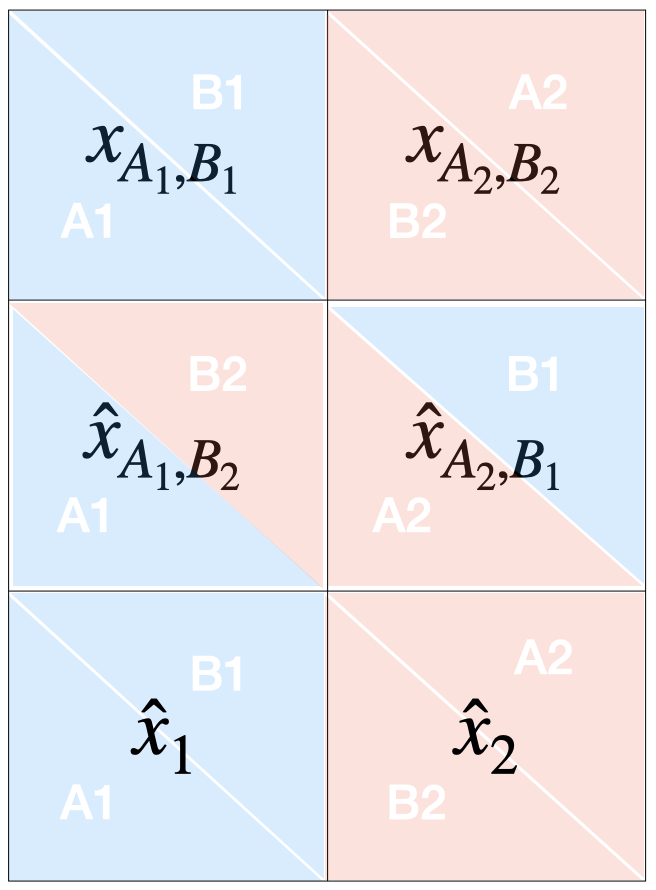
\includegraphics[width=0.5\linewidth]{figures/layout.png}
	\caption{Plot Layout of original (first row), mixed (second row) and reconstructed images (third row)}
	\label{fig:plot_layout}
\end{figure}

\begin{figure}[h!]
	\centering
	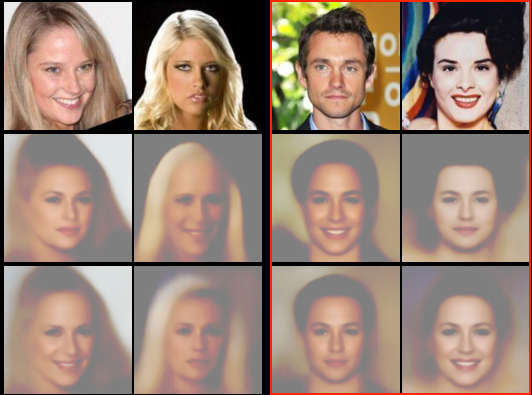
\includegraphics[width=\linewidth]{figures/naive_res.png}
	\caption{Results of naive approach (Epochs: 20, Batch Size: 32, $\gamma = 0.4$)}
	\label{fig:naive_results}
\end{figure}

\subsection{CycleFUNIT}
The experimental results of the CycleFUNIT approach are subdivided into the two major experiments. In the first experiment, we use the FUNIT architecture assembled into the G2G structure with the CycleGAN objective. The loss is a combination of the "long" reconstruction loss, the cycle consistency losses, and the GAN loss. The results in figure \ref{fig:cycle_funit_results} show that the network simply copies the image through and this approach fails to achieve disentanglement.

\begin{figure}[h!]
	\centering
	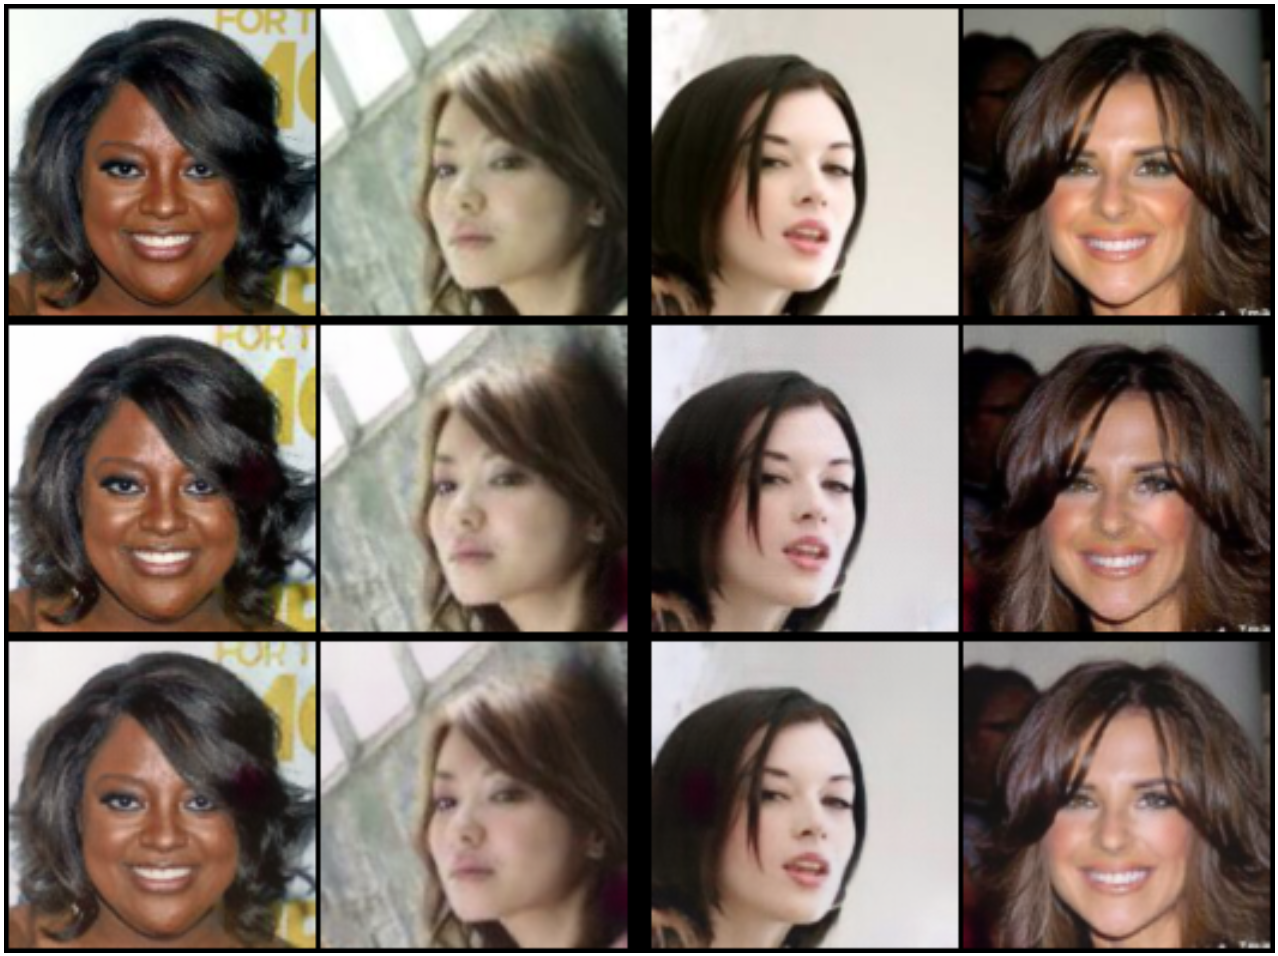
\includegraphics[width=\linewidth]{figures/cycle_funit.png}
	\caption{Results of CycleFUNIT approach (Epoch: 124, Batch Size: 4)}
	\label{fig:cycle_funit_results}
\end{figure}

In a second stage, we added the pre-trained identity encoder. First, we used it to encode the identity of the mixed images. This strongly disturbed the training of our generative model and resulted in mode collapse. We thought that the problem that causes this is that we add the identity loss in equation \ref{eq:cyclefunit_id} from the very beginning when the generated images are still random pixels. We tried to linearly increase the weight of the identity loss. This was not successful and we obtained the same results as in figure \ref{fig:cycle_funit_results}.
When we replaced encoder $E_B$ with the identity encoder we faced issues with adversarial samples. The cycle consistency loss $\mathcal{L}_{cyc, E_B}$ -- which is the new identity loss -- rapidly reduced to near-zero (within the first 50 iterations), but the results still stayed the same as in figure \ref{fig:cycle_funit_results}. This suggests that the loss over the pre-trained identity encoder is "tricked" by adversarial samples -- some image features that lead to a rapid decrease of the identity cycle consistency loss. Reducing the weight of the identity loss (making it less of an objective to minimize right from the start) was not successful. Furthermore, we also reduced the size of the content code to increase the importance of the identity code by introducing more downsampling steps in the FUNIT content encoder. However, this did also not yield better results. 

\subsection{FUNIT2FUNIT}
For all experiments, we resumed training from the pre-trained network by Liu et al. which is trained until the 149th epoch. First, we perform our cross-forward feed which wires the encoders to the decoders according to figure \ref{fig:funit2funit}. A simple forward pass gives the results seen in figure \ref{fig:cross}. These results feature very good image quality and achieve good disentanglement of class and content information. It should be noted that the reconstructions are slightly different compared to the original images. We aim to improve these results by resuming training from this point onward. 

\begin{figure}[h!]
	\centering
	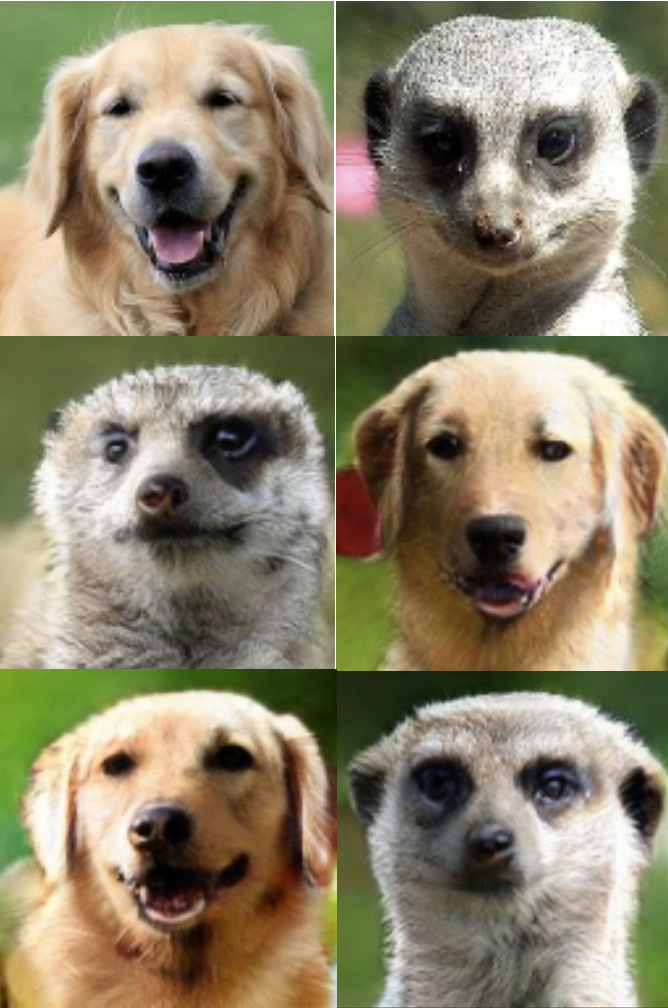
\includegraphics[width=0.5\linewidth]{figures/funit_cross_forward_pass.png}
	\caption{A simple forward pass through the pre-trained FUNIT2FUNIT model}
	\label{fig:cross}
\end{figure}

To the vanilla FUNIT losses we iteratively added the modifications, we described in section \ref{chap4_methods_FUNIT2FUNIT}, starting with the long L1 reconstruction loss. The results we obtained by adding the long reconstruction loss with $\lambda_{L}=0.1$ can be seen in figure \ref{fig:imgs_long_recon}. The batch size of all FUNIT2FUNIT experiments is 4.

\begin{figure}[h!]
	\centering
	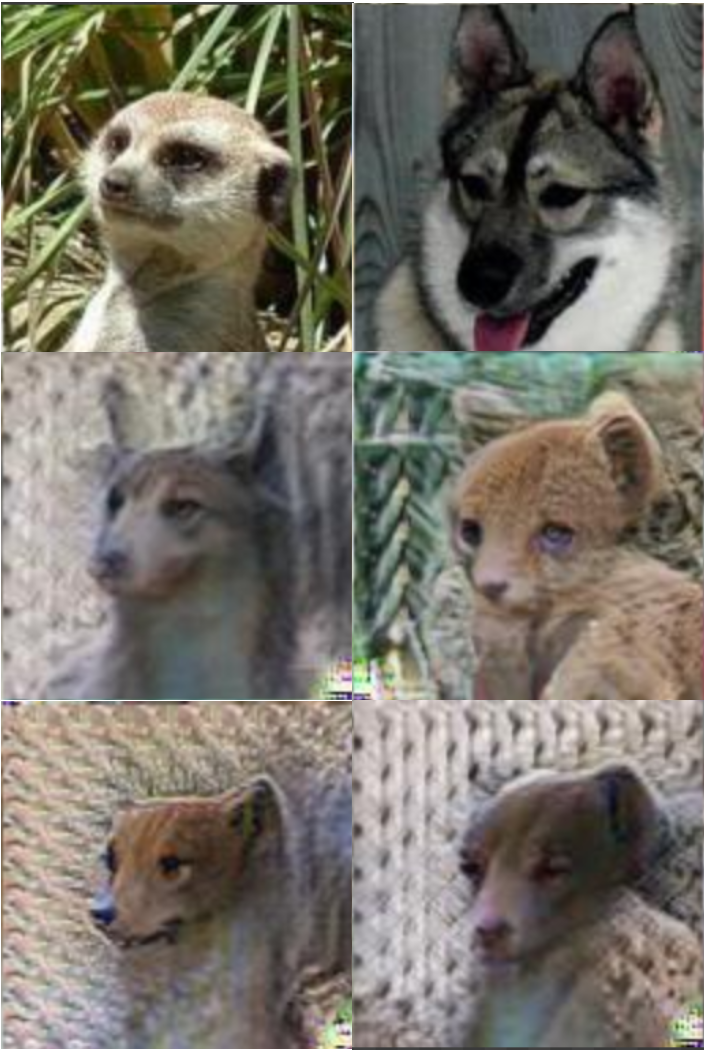
\includegraphics[width=0.5\linewidth]{figures/long_recon_0'1.png}
    \caption{Results after adding a long reconstruction loss with $\lambda_{L}=0.1$}
    \label{fig:imgs_long_recon}
\end{figure}

In the second iteration, the feature matching loss is extended by the long-range loss and the reassembly stage loss. $\lambda_{D}$ is set to 1.0 in the original FUNIT approach and we leave this value unchanged. $\lambda_{R}$ is set to 0.1 to prevent the losses from rapidly jumping to a high level. This gave the qualitative results depicted in figure \ref{fig:funit2funit_all_losses}.

\begin{figure}[h!]
	\centering
	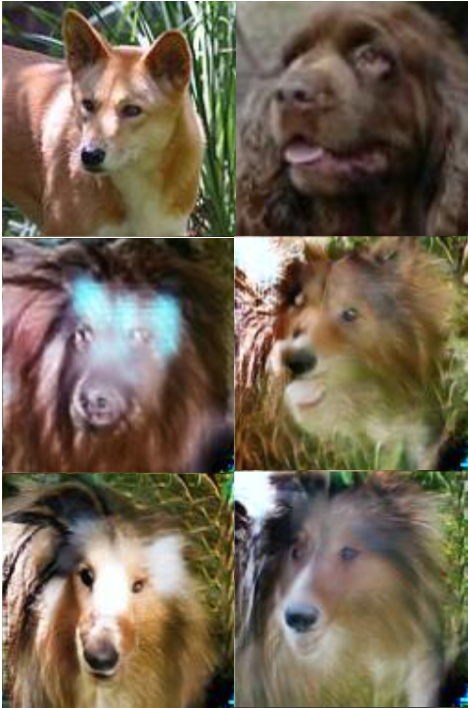
\includegraphics[width=0.5\linewidth]{figures/funit2funit_all_losses.png}
	\caption{Results after 10 iterations using all losses in equation \ref{eq:funit2funit_overall}}
	\label{fig:funit2funit_all_losses}
\end{figure}

Unfortunately, instead of improving disentanglement quality, the images degrade in quality after a few iterations. A reason for this may be that the optimization objective is too complex and the additional losses we introduced (long reconstruction loss, long feature matching loss, and reassembly stage feature matching loss) skew the original results. This has to be further scrutinized.

\label{chap6_discussion}
\section{Discussion and Outlook}
The research question in the focus of this project is evaluating the impact of the proposed G2G architecture on the disentanglement of image features. To reach the disentanglement of the class and content information we first set up the network from scratch in a naive approach. Due to lacking photo-realism and image quality we then leveraged the FUNIT architecture by Liu et al. in our second approach. This resulted in better image quality but no disentanglement. However, this approach seems worth investigating more deeply: the problem of adversarial samples needs to be addressed further from an architectural standpoint. We believe that the content information is too dominant, hence the class information is ignored. In future work, it should be investigated how we can guide the network to put more emphasis on the identity code. The size of the latent FUNIT content code should be reduced such that the network must also use the identity information to satisfy the losses. Simply including more downsampling layers in the content encoder is not sufficient as it dramatically increases network size. Bigger kernel sizes and higher strides may be useful for reducing the size of the latent code quickly.

The third approach solely focuses on answering the research question at hand -- to find out whether the G2G architecture helps disentanglement or not. We believe that extending the experiments for the third approach can give more answers on whether this is the case, even though our first attempts at resuming training of the pre-trained networks were difficult. An important contribution of our work is that we proved that a forward pass through the FUNIT2FUNIT architecture produces sensible results. However, when resuming training the FUNIT2FUNIT approach seems to have difficulties satisfying the newly introduced losses with the pre-trained networks. An ablation study could be performed with the new losses to see which losses lead to the rapid degradation in image quality. Namely, these are the long reconstruction loss, the long feature matching loss, and the feature matching loss between the mixed and the fully reconstructed images. 

Another, approach which is not directly linked to answering the research question but is a promising approach to achieve disentangled features is erasing identity-sensitive information of the content images. More specifically, facial features such as eyes, nose, and mouth could be erased which would force the content encoder to encode common information such as pose, background, and lighting. The other encoder would be fed with an unmodified image, of which the identity-sensitive information is then encoded.

\label{chap7_conclusion}
\section{Conclusion}
In this project, we described three independent attempts at disentangling class and content information with the G2G architecture. We compare these different approaches with each other and conclude that the FUNIT architecture is more powerful than the LORD generator in generating highly realistic images. However, we also found that disentangling image features with the G2G architecture is a challenging task in the first two approaches. 

By performing a forward pass through the pre-trained FUNIT2FUNIT network we demonstrated that the principle behind G2G works: we can mix content and class information and successfully reconstruct an image that looks similar to the original. However, we also found that resuming training for the FUNIT2FUNIT approach is challenging. We proposed several ideas for future work, which may help other researchers in achieving disentanglement from the considerations which we presented in this project.

\section*{Acknowledgment}
The authors would like to thank Ron Mokady, Daniel Cohen-Or, and Yotam Nitzan for their ongoing support during the Machine Learning Applications for Computer Graphics course at Tel Aviv University. We hope to stay in touch in the future and extend this project further in collaboration with you.

\printbibliography

\end{document}